\documentclass{article}
\usepackage[utf8]{inputenc}
\usepackage{amssymb, amsmath, amsthm}
\usepackage{thmtools, mathtools, mathrsfs}
\usepackage{amsfonts}
\usepackage[sort&compress,numbers]{natbib}
\usepackage{subcaption}
\usepackage{graphicx}
\usepackage{caption}
\usepackage{float}
\usepackage{bm}
\usepackage{tikz}
\usetikzlibrary{positioning,matrix,arrows,decorations.pathmorphing}
\usepackage{tikz-cd} 
\definecolor {processblue}{cmyk}{0.8,0,0,0}

\newcommand{\mb}[1]{\mathbb{#1}}
\newcommand{\mc}[1]{\mathcal{#1}}
\DeclareMathOperator{\Inv}{Inv}
\DeclareMathOperator{\innt}{int}
\newcommand{\probP}{\text{I\kern-0.15em P}}

\newtheorem{theorem}{Theorem}
\newtheorem{prop}{Proposition}
\theoremstyle{definition}
\newtheorem{definition}{Definition}
\theoremstyle{remark}
\newtheorem{remark}{Remark}

 \usepackage{thmtools, thm-restate} \newtheorem{conjecture}[theorem]{Conjecture}

\title{}
\author{\'Abel S\'agodi}
\date{April 1, 2023}

\begin{document}
\maketitle

Here, we show the implementation of a system with two fixed points in an S4 network with two layers.
Each layer has a single node.

The weight in the first layer can be chose to be positive (which is in line with the HIPPO matrix definition).

In this case the network will converge to positive or negative infinity, depending on the inputs (mostly the initial inputs),
\[x(t) \rightarrow \pm \infty.\]

If we use  tanh function for the non-linearity,
for example by choosing $u(t) = \alpha\tanh(x) + \beta$,
we can let the input of the next layer go to 
\begin{equation}
u(t) \rightarrow
\begin{cases}
a = \alpha + \beta & \text{ for }  x(t)\rightarrow \infty\\
b = \alpha - \beta& \text{ for }  x(t)\rightarrow -\infty.
\end{cases}
\end{equation}

This in turn gives two fixed points in the second layer: $x_1^*=-a$ and $x_2^*=-b$.



\begin{conjecture}\label{universality}
With the number of layers going to infinity, we can approximate a topologically conjugate version of any dynamical system with a finite number of fixed points. 
\end{conjecture}


\section{Linear-Nonlinear tanh system}

\begin{definition}
\begin{align}
\dot x &= Ax\\
       y &= f(x)
\end{align}
where $x\in\mathbb{R}^n$, $y\in\mathbb{R}^m$ and $f\colon \mathbb{R}^n\rightarrow\mathbb{R}^m$.
\end{definition}

\begin{remark}
This system can be rewritten as $\dot y = g(y)$ for some $g\colon\mathbb{R}^m\rightarrow\mathbb{R}^m$.
\end{remark}

We look at a linear-nonlinear dynamical system that has some interesting property, i.e., it is not equivalent to any linear dynamical system.

\begin{align}
\dot x &= \alpha x\\
       y &= \tanh(x)
\end{align}

\begin{align*}
\dot y &= \frac{d \tanh(x)}{dx}\frac{dx}{dt}\\
&= \frac{\alpha x}{\cosh^2(x)}\\
&=  \frac{\alpha \tanh^{-1}(y)}{\cosh^2( \tanh^{-1}(y))}\\
&= \alpha(1-y^2) \tanh^{-1}(y)
\end{align*}




\begin{figure}[H]
 \centering
 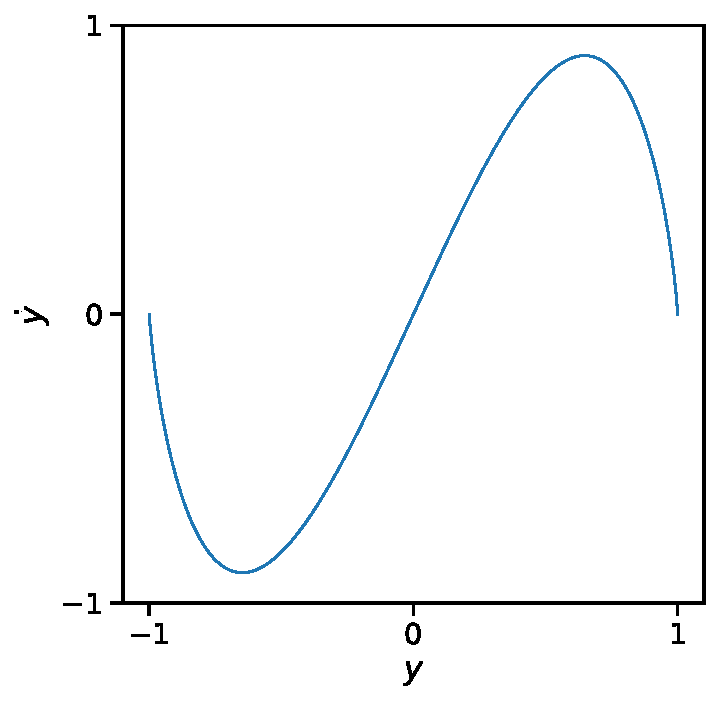
\includegraphics[width=0.99\textwidth]{figs/tanh_ydot.pdf}
 \caption{}
 \label{fig:tanh_ydot}
\end{figure}


\begin{equation}
\frac{g(y)}{dy} = 1 - 2 y \tanh^{-1}(y)
\end{equation}



\begin{figure}[H]
 \centering
 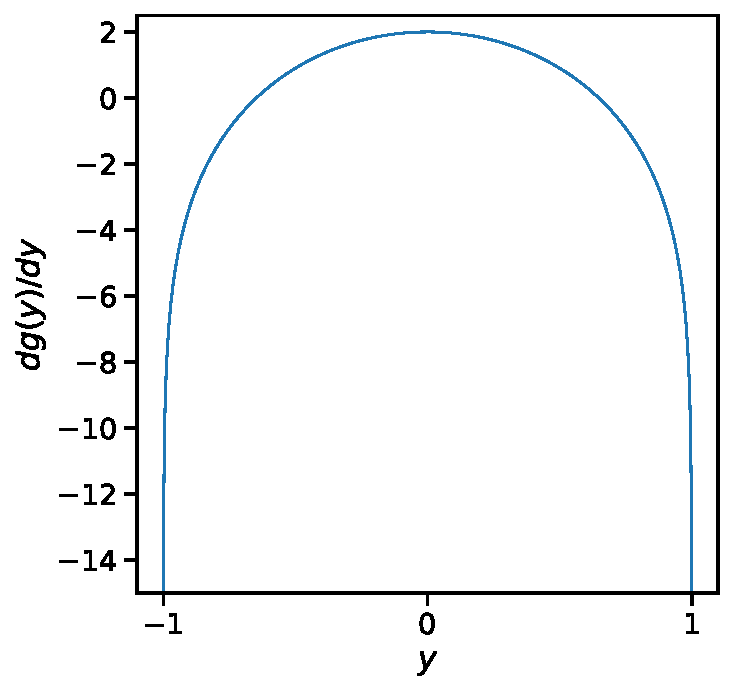
\includegraphics[width=0.99\textwidth]{figs/tanh_dydot.pdf}
 \caption{}
 \label{fig:tanh_dydot}
\end{figure}

% \newpage
% \addcontentsline{toc}{section}{References}
% \bibliographystyle{plain}
% \bibliography{CIT-for-Computation.bib, cit.bib, CITCOD.bib}

\end{document}